\documentclass[conference]{IEEEtran}
\IEEEoverridecommandlockouts

\usepackage[backend=biber]{biblatex}
\addbibresource{references.bib}
\usepackage{amsmath,amssymb,amsfonts}
\usepackage{algorithmic}
\usepackage{graphicx}
\usepackage{textcomp}
\usepackage{xcolor}
\usepackage{listings}
\usepackage{booktabs}
\usepackage{hyperref}
\usepackage{cleveref}

% TikZ for diagrams
\usepackage{tikz}
\usetikzlibrary{shapes.geometric, arrows.meta, positioning, shadows, fit, backgrounds}

% YAML listing style
\lstdefinestyle{yaml}{
  basicstyle=\ttfamily\footnotesize,
  breaklines=true,
  frame=single,
  numbers=left,
  numberstyle=\tiny\color{gray},
  keywordstyle=\color{blue},
  stringstyle=\color{orange},
  commentstyle=\color{gray},
  showstringspaces=false,
  tabsize=2
}

\def\BibTeX{{\rm B\kern-.05em{\sc i\kern-.025em b}\kern-.08em
    T\kern-.1667em\lower.7ex\hbox{E}\kern-.125emX}}

\begin{document}

\title{TMDL: A Description Language for Virtual TeamMates in Hybrid Human-AI Teams}

\author{
    \IEEEauthorblockN{Pedro A. Pernías Peco}
    \IEEEauthorblockA{
        Departamento de Lenguajes y Sistemas Informáticos\\
        Universidad de Alicante\\
        Alicante, España\\
        p.pernias@ua.es
    }
    \and
    \IEEEauthorblockN{M. Pilar Escobar Esteban}
    \IEEEauthorblockA{
        Departamento de Lenguajes y Sistemas Informáticos\\
        Universidad de Alicante\\
        Alicante, España\\
        pilar.escobar@ua.es
    }
}

\maketitle

\begin{abstract}
The integration of Large Language Models (LLMs) into collaborative work environments presents a fundamental design choice: should AI function as a \textit{tool} for ad-hoc queries or as a \textit{teammate} with defined identity and role? This paper introduces TMDL (TeamMate Description Language), a YAML-based specification language for describing virtual TeamMates in hybrid human-AI teams. Building on ADL (Assistant Description Language), the ``machines as teammates'' research agenda, and organizational behavior research on team effectiveness, TMDL provides structured specifications for identity, role, collaboration patterns, and project knowledge. Key contributions include: (1) a contribution-centered collaboration model that frames AI TeamMates around how they add value to the group; (2) taxonomies for contribution styles and cognitive patterns derived from established team composition research; and (3) explicit boundary specifications that position AI as a configured partner operating under human direction. We derive six research hypotheses comparing the teammate paradigm against tool-based AI use and propose a quasi-experimental validation approach. The specification is released as open-source at \url{https://github.com/ppernias/tmdl}.
\end{abstract}

\begin{IEEEkeywords}
Large Language Models, Human-AI Collaboration, Agent Description Languages, Virtual Teams, Prompt Engineering
\end{IEEEkeywords}

% ==============================================================================
\section{Introduction}
% ==============================================================================

The rapid advancement of Large Language Models (LLMs) has opened unprecedented opportunities for human-AI collaboration in professional and academic settings. However, deploying LLMs as effective team members rather than mere tools presents unique challenges that go beyond traditional prompt engineering approaches.

When humans collaborate in teams, they bring not only their skills but also their personalities, communication styles, and understanding of team dynamics. Research on AI as teammates has identified significant open challenges in this integration---including role distribution, trust dynamics, and coordination patterns---that fundamentally differ from traditional tool-based human-computer interaction \cite{seeber2020machines}.

Consider a project team where an AI agent is expected to serve as a research analyst. Beyond answering questions, the agent must understand its role boundaries, know when to defer to others, maintain consistent communication patterns, and adapt its behavior to project phases and team needs. Encoding all these requirements in unstructured natural language prompts leads to several problems: ambiguity in interpretation, prompt drift as specifications evolve, lack of validation mechanisms, and poor reproducibility across deployments.

This paper introduces TMDL (TeamMate Description Language), an evolution of ADL (Assistant Description Language) \cite{pernias2025adl} specifically designed for team collaboration contexts. TMDL addresses these challenges by providing:

\begin{itemize}
    \item A \textbf{formal schema} for describing AI TeamMates with consistent structure and validation
    \item \textbf{Separation of concerns} between identity, role, collaboration patterns, and project knowledge
    \item \textbf{Theoretically-grounded taxonomies} for contribution styles and cognitive patterns
    \item A \textbf{contribution-centered collaboration model}, grounded in team effectiveness research, that frames TeamMates around how they add value to the group
    \item \textbf{Protocol-based behavior} specification for predictable responses to team events
\end{itemize}

Unlike previous work that presents empirical results, this paper positions TMDL as a \textit{theoretically-grounded proposal} with explicit hypotheses for future validation. We derive our design decisions from the ``machines as teammates'' research agenda \cite{seeber2020machines}, team effectiveness models from organizational behavior \cite{ilgen2005teams}, and recent work on collective human-machine intelligence \cite{gonzalez2023cohumain}, articulating testable predictions comparing AI-as-teammate against AI-as-tool paradigms.

The remainder of this paper is organized as follows: Section II presents the theoretical foundations underlying TMDL's design, including the critical distinction between tool and teammate paradigms. Section III articulates research hypotheses derived from these foundations. Section IV describes the TMDL architecture. Section V details the schema specification. Section VI provides an illustrative example. Section VII discusses implications and limitations. Section VIII concludes with future directions.

% ==============================================================================
\section{Theoretical Foundations}
% ==============================================================================

TMDL's design draws from three research streams that converge to provide a comprehensive theoretical foundation (Figure~\ref{fig:tmdl-foundations}). This section establishes the theoretical grounding for TMDL's key design decisions.

% TMDL Theoretical Foundations Diagram (sized for IEEE single column)
\begin{figure}[htbp]
\centering
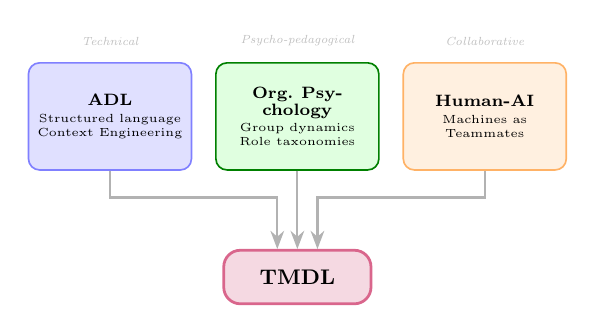
\begin{tikzpicture}[scale=0.85, every node/.style={scale=0.85},
    % Styles
    pillar/.style={
        rectangle,
        rounded corners=4pt,
        minimum width=2.4cm,
        minimum height=1.6cm,
        text width=2.2cm,
        align=center,
        font=\tiny
    },
    adl/.style={pillar, fill=blue!12, draw=blue!50, line width=0.6pt},
    psych/.style={pillar, fill=green!12, draw=green!50!black, line width=0.6pt},
    hai/.style={pillar, fill=orange!12, draw=orange!60, line width=0.6pt},
    result/.style={
        rectangle,
        rounded corners=6pt,
        minimum width=2.2cm,
        minimum height=0.8cm,
        align=center,
        fill=purple!15,
        draw=purple!60,
        line width=1pt,
        font=\small\bfseries
    },
    arrow/.style={
        ->,
        >=Stealth,
        line width=0.8pt,
        color=gray!60
    },
    label/.style={
        font=\tiny\itshape,
        text=gray!50
    }
]

% Three pillars
\node[adl] (adl) at (0,0) {
    \textbf{\scriptsize ADL}\\[1pt]
    Structured language\\
    Context Engineering
};

\node[psych] (psych) at (2.8,0) {
    \textbf{\scriptsize Org. Psychology}\\[1pt]
    Group dynamics\\
    Role taxonomies
};

\node[hai] (hai) at (5.6,0) {
    \textbf{\scriptsize Human-AI}\\[1pt]
    Machines as\\
    Teammates
};

% Result node
\node[result] (tmdl) at (2.8,-2.4) {TMDL};

% Arrows
\draw[arrow] (adl.south) -- ++(0,-0.4) -| ([xshift=-0.3cm]tmdl.north);
\draw[arrow] (psych.south) -- (tmdl.north);
\draw[arrow] (hai.south) -- ++(0,-0.4) -| ([xshift=0.3cm]tmdl.north);

% Labels for foundations
\node[label, above=0.1cm of adl] {Technical};
\node[label, above=0.1cm of psych] {Psycho-pedagogical};
\node[label, above=0.1cm of hai] {Collaborative};

\end{tikzpicture}
\caption{TMDL theoretical foundations: three research streams converging into the TeamMate Description Language.}
\label{fig:tmdl-foundations}
\end{figure}

\subsection{Technical Foundation: ADL and Structured Prompting}

TMDL is a direct evolution of ADL (Assistant Description Language) \cite{pernias2025adl}, inheriting its core architecture while extending it for team collaboration. Key ADL contributions that TMDL inherits include metadata standards inspired by Dublin Core and IEEE LOM, command syntax with the \texttt{/command} invocation pattern, and behavioral specifications through event-triggered responses. ADL was designed for general-purpose conversational assistants focusing on single-user interactions; TMDL extends this foundation to multi-party team contexts, adding constructs for role definition, collaboration patterns, and team dynamics.\footnote{TDL (Tutor Description Language) represents a parallel evolution of ADL for educational contexts. Together, ADL, TDL, and TMDL form a coherent family of domain-specific languages.}

Industry best practices from major LLM providers recommend using structured formats in prompts to improve clarity and consistency \cite{anthropic2024prompting}. Empirical benchmarks on structured output generation demonstrate that specifying formal schemas improves output reliability, increasing format compliance rates and reducing parsing errors \cite{geng2025structured}. Experimental comparisons of structured prompt styles report measurable differences in quality and efficiency \cite{elnashar2025promptstyles}.

Khattab et al. \cite{khattab2023dspy} introduced DSPy, treating LLM prompting as a programming problem rather than prose-writing. Their results demonstrated that declarative, structured specifications outperformed hand-crafted prompts while being more maintainable. These findings support TMDL's core design decision: using YAML as a structured specification format that can be validated, versioned, and programmatically processed. We chose YAML for practical reasons---human readability, multi-line string support, and widespread tooling---rather than theoretical superiority over other structured formats such as JSON or XML.

\subsection{Psycho-pedagogical Foundation: Team Effectiveness and Role Theory}

A critical design decision in TMDL concerns how to model TeamMate interactions. Research on team effectiveness provides clear guidance: high-performing teams are characterized by coordination, mutual support, and shared purpose.

Hackman's team effectiveness model \cite{hackman2002leading} identifies shared leadership and enabling structure as key drivers of team performance. Salas et al.'s ``Big Five'' of teamwork \cite{salas2005bigfive} highlights mutual performance monitoring and backup behavior---fundamentally cooperative mechanisms where teammates anticipate each other's needs and provide support proactively. Research shows that high-performing teams are characterized by role clarity and task interdependence \cite{widianto2024task}. Task interdependence naturally promotes coordination, trust, and information sharing. When team members depend on each other to accomplish work, they develop shared understanding and effective collaboration patterns.

This research foundation leads directly to TMDL's design: a \textit{contribution-centered} model that asks ``How does this TeamMate add value to the group?'' By focusing on positive contribution patterns---supporting others, generating ideas, analyzing proposals, integrating perspectives, driving execution---TMDL aligns with how effective teams actually function.

TMDL's taxonomies are derived from established organizational behavior research rather than invented \textit{ad hoc}:

\textbf{Contribution Style Taxonomy.} TMDL defines five contribution styles grounded in team composition research. Mathieu et al. \cite{mathieu2014composition} demonstrate that effective teams require heterogeneity in task-relevant attributes---competencies, experiences, and behavioral orientations---with different compositional configurations optimal for different work phases. Earlier, Benne and Sheats \cite{benne1948functional} established the foundational distinction between task-oriented and maintenance-oriented functional roles in groups. Building on this research, TMDL's contribution styles capture the primary ways TeamMates add value: \texttt{supportive} (enabling others' contributions), \texttt{generative} (generating ideas), \texttt{analytical} (evaluating proposals), \texttt{integrative} (synthesizing perspectives), and \texttt{executive} (driving execution).

\textbf{Cognitive Style Taxonomy.} Research on cognitive styles provides a rigorous foundation for differentiating thinking patterns. Kirton's Adaption-Innovation theory \cite{kirton1976adaptors} established a fundamental dimension validated across decades of research: \textit{adaptors} who improve within existing paradigms versus \textit{innovators} who challenge and transform them. Critically, Aggarwal and Woolley \cite{aggarwal2019cognitive} demonstrated empirically that cognitive style diversity in teams improves collective performance through enhanced team cognition. TMDL operationalizes Kirton's continuum through three cognitive style values: \texttt{adaptor}, \texttt{innovator}, and \texttt{balanced}. These are not personality traits but assignable cognitive orientations that can be deliberately configured to create complementary team compositions.

\subsection{Collaborative Foundation: Human-AI Teaming Research}

A fundamental distinction in human-AI collaboration concerns whether AI systems are conceptualized as \textit{tools} or as \textit{teammates}. This distinction has significant implications for system design, user expectations, and collaboration outcomes.

Seeber et al. \cite{seeber2020machines} established the research agenda for ``machines as teammates,'' asking: ``What if AI machines became teammates rather than tools?'' Their work identifies that for AI to function as a teammate, it must perform a unique role, make unique contributions, and participate in coordination with human team members. This framing---AI as an active participant rather than passive instrument---forms the foundation of TMDL's design philosophy.

Empirical evidence supports the practical importance of this distinction. Goh et al. \cite{goh2025tooltoteammate} conducted a randomized controlled trial comparing clinicians using AI as a ``collaborative teammate'' versus as a ``traditional tool.'' The teammate condition achieved significantly higher diagnostic accuracy (85\% vs. 75\%, p < 0.001), with qualitative analysis revealing greater engagement and more effective integration of AI contributions.

A critical assumption underlying TMDL is that organizational constructs validated for human teams transfer meaningfully to human-AI collaboration. Recent research provides qualified support: Lou et al. \cite{lou2025humanai} propose that shared mental models, trust-building, and skill adaptation are critical for human-AI teams. However, this transfer requires acknowledgment of key differences. Bansal et al. \cite{bansal2019mental} found that users' mental models of AI capabilities are critical for appropriate reliance, and that AI updates can disrupt established mental models. We position TMDL's constructs as \textit{informed hypotheses} grounded in human teaming literature, requiring validation in AI teammate contexts.

Recent work on collective human-machine intelligence \cite{gonzalez2023cohumain} further refines this paradigm, cautioning against treating AI ``like any other teammate'' and instead positioning it as a \textit{partner that works under human direction}---capable of strengthening human capabilities while operating within defined boundaries. TMDL positions itself firmly within the ``teammate'' paradigm, but with important qualifications: TeamMates are \textit{configured} (not autonomous), have \textit{bounded capabilities} (explicit limitations), are \textit{deferential by design} (human authority preserved), and have \textit{no ego to protect} (purely constructive contribution).

We use ``teammate'' throughout this paper in this specific sense: a collaborative entity with defined identity, role, and contribution patterns, operating under human direction within explicit boundaries. This framing enables the benefits of teammate-style collaboration (engagement, integration, role clarity) while maintaining appropriate expectations about AI capabilities.

% ==============================================================================
\section{Research Hypotheses}
% ==============================================================================

Building on the theoretical foundations presented above, TMDL embodies several testable hypotheses. These hypotheses are formulated to compare AI integration paradigms: \textit{AI as teammate} (using TMDL specifications) versus \textit{AI as tool} (using AI for ad-hoc queries without structured teammate configuration).

\subsection{Hypotheses on the Teammate Paradigm}

\textbf{H1 (Behavioral Consistency):} Teams using TMDL-defined AI TeamMates will experience higher behavioral consistency in AI responses than teams using AI as a generic tool.

\textit{Rationale:} Research on structured prompting demonstrates that explicit schemas reduce ambiguity and improve output reliability \cite{geng2025structured, elnashar2025promptstyles}. When AI is used as a tool without persistent configuration, each interaction starts without accumulated context, leading to inconsistent behavior patterns. TMDL's structured specifications should produce more predictable TeamMate behavior.

\textbf{H2 (Role Clarity Effect):} Teams working with TMDL-defined TeamMates will report higher role clarity and fewer expectation violations than teams using AI as a tool.

\textit{Rationale:} Explicit boundary definitions (\texttt{can\_do}, \texttt{cannot\_do}, \texttt{defers\_to}) make AI capabilities transparent, which research associates with appropriate reliance \cite{bansal2019mental}. Tool-based AI use lacks explicit role definition, potentially leading to unclear expectations about what the AI can contribute.

\textbf{H3 (Team Integration Quality):} TMDL-configured AI TeamMates will be perceived as more integrated team members than AI used in tool mode, as measured by team cohesion and collaboration quality scales.

\textit{Rationale:} Research on machines as teammates \cite{seeber2020machines} and empirical evidence \cite{goh2025tooltoteammate} suggest that positioning AI as a collaborative partner rather than a tool improves engagement and integration outcomes. TMDL's identity, personality, and protocol specifications operationalize this TeamMate positioning.

\subsection{Hypotheses on Contribution Patterns}

\textbf{H4 (Contribution-Centered Dynamics):} Teams using TMDL TeamMates with defined contribution styles will exhibit more structured collaboration patterns than teams using AI as an undifferentiated tool.

\textit{Rationale:} Research on high-performing teams emphasizes coordination and role complementarity \cite{salas2005bigfive, mathieu2014composition}. TMDL's contribution-centered model explicitly configures how TeamMates add value, while tool-based AI use provides no such structure.

\textbf{H5 (Behavioral Differentiation):} Different contribution styles and cognitive styles specified in TMDL will produce measurably different AI behaviors within the same team context.

\textit{Rationale:} If organizational behavior constructs transfer validly to AI TeamMates, specifying \texttt{contribution\_style: analytical} versus \texttt{supportive} should produce observably different interaction patterns. This tests construct validity independently of tool-versus-teammate comparisons.

\textbf{H6 (Composition Effects):} Teams with complementary TMDL-defined contribution styles (e.g., analytical + generative) will outperform teams with homogeneous styles on complex collaborative tasks.

\textit{Rationale:} Cognitive diversity research demonstrates that diverse thinking styles improve collective intelligence \cite{aggarwal2019cognitive, woolley2010collective}. This should extend to AI TeamMate composition within TMDL-configured teams.

\subsection{Validation Approach}

These hypotheses will be tested through a quasi-experimental design comparing:

\begin{itemize}
    \item \textbf{Experimental condition}: Teams using TMDL-defined AI TeamMates with explicit identity, role, contribution style, and project context
    \item \textbf{Comparison condition}: Teams using AI as a generic tool for ad-hoc queries without structured teammate configuration
\end{itemize}

This design reflects the practical reality that ``no AI'' control groups are increasingly infeasible in educational and professional settings. The comparison captures the meaningful distinction between paradigms: AI integrated as a configured team member versus AI accessed as an external resource.

Metrics will include: behavioral consistency (response pattern analysis), role clarity (validated scales), team integration (cohesion measures), collaboration quality (process observation), and task performance on semester-long project outcomes. H5 and H6 will be tested within the experimental condition by varying TeamMate configurations.

% ==============================================================================
\section{TMDL Architecture}
% ==============================================================================

\subsection{Design Principles}

TMDL is designed around six core principles:

\begin{enumerate}
    \item \textbf{Structured over Unstructured}: Following industry best practices \cite{anthropic2024prompting}, TMDL uses YAML schemas rather than free-form text, enabling validation and reducing ambiguity.

    \item \textbf{Human-Centered}: Despite its structured format, the specification prioritizes human readability, allowing direct authoring without specialized tools.

    \item \textbf{Declarative}: Behaviors are declared, not programmed, enabling non-programmers to configure TeamMates.

    \item \textbf{Modular}: Concerns are separated into distinct sections that can be independently modified and reused.

    \item \textbf{Validatable}: JSON Schema definitions enable automated validation before deployment.

    \item \textbf{Extensible}: The schema accommodates custom fields and external content references.
\end{enumerate}

\subsection{Contribution-Centered Collaboration Model}

A key design decision concerns how to model TeamMate interactions. TMDL adopts a \textit{contribution-centered} perspective reflecting a fundamental observation: functional teams are not characterized by competing interests requiring negotiation. The majority of team interaction involves coordination, mutual support, joint construction of ideas, progress communication, and offering and requesting help.

TMDL therefore asks: ``How does this TeamMate add value to the group?'' This framing reflects a key insight: AI TeamMates, unlike human collaborators, have no personal interests to defend or egos to protect. They can be configured purely for constructive contribution.

\subsection{Overall Structure}

A TMDL document consists of five main sections plus metadata, organized into static TeamMate definition and dynamic context (Figure~\ref{fig:tmdl-structure}):

% TMDL Structure Diagram
\begin{figure}[htbp]
\centering
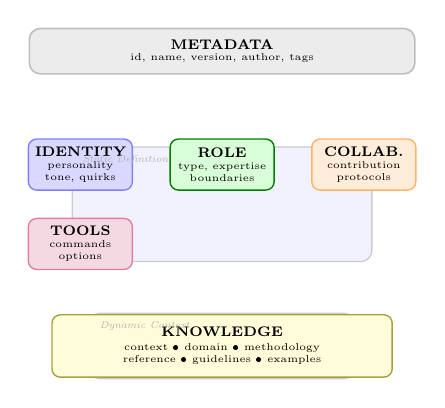
\begin{tikzpicture}[scale=0.72, every node/.style={scale=0.72},
    % Styles
    section/.style={
        rectangle,
        rounded corners=3pt,
        minimum height=0.9cm,
        text width=1.6cm,
        align=center,
        font=\tiny
    },
    metadata/.style={
        rectangle,
        rounded corners=4pt,
        fill=gray!15,
        draw=gray!50,
        line width=0.6pt,
        minimum width=6.8cm,
        minimum height=0.8cm,
        align=center,
        font=\tiny
    },
    groupbox/.style={
        rectangle,
        rounded corners=4pt,
        draw=gray!40,
        line width=0.5pt,
        inner sep=4pt
    },
    grouplabel/.style={
        font=\tiny\itshape,
        text=gray!60
    },
    identity/.style={section, fill=blue!15, draw=blue!50, line width=0.5pt},
    role/.style={section, fill=green!15, draw=green!50!black, line width=0.5pt},
    collab/.style={section, fill=orange!15, draw=orange!60, line width=0.5pt},
    tools/.style={section, fill=purple!15, draw=purple!50, line width=0.5pt},
    knowledge/.style={
        rectangle,
        rounded corners=3pt,
        fill=yellow!15,
        draw=yellow!60!black,
        line width=0.5pt,
        minimum width=6cm,
        minimum height=1.1cm,
        align=center,
        font=\tiny
    }
]

% METADATA section
\node[metadata] (meta) at (3.4, 4.8) {
    \textbf{\scriptsize METADATA}\\
    id, name, version, author, tags
};

% Static definition group
\node[identity] (identity) at (0.9, 2.8) {
    \textbf{\scriptsize IDENTITY}\\
    personality\\
    tone, quirks
};

\node[role] (role) at (3.4, 2.8) {
    \textbf{\scriptsize ROLE}\\
    type, expertise\\
    boundaries
};

\node[collab] (collab) at (5.9, 2.8) {
    \textbf{\scriptsize COLLAB.}\\
    contribution\\
    protocols
};

\node[tools] (tools) at (0.9, 1.4) {
    \textbf{\scriptsize TOOLS}\\
    commands\\
    options
};

% Background for static
\begin{scope}[on background layer]
    \node[groupbox, fill=blue!5, fit=(identity)(role)(collab)(tools), inner sep=5pt] (staticbox) {};
\end{scope}
\node[grouplabel, anchor=north west] at ([xshift=2pt, yshift=-1pt]staticbox.north west) {Static Definition};

% Knowledge section (dynamic)
\node[knowledge] (know) at (3.4, -0.4) {
    \textbf{\scriptsize KNOWLEDGE}\\[1pt]
    context \textbullet{} domain \textbullet{} methodology\\
    reference \textbullet{} guidelines \textbullet{} examples
};

% Background for dynamic
\begin{scope}[on background layer]
    \node[groupbox, fill=yellow!5, fit=(know), inner sep=5pt] (dynbox) {};
\end{scope}
\node[grouplabel, anchor=north west] at ([xshift=2pt, yshift=-1pt]dynbox.north west) {Dynamic Context};

\end{tikzpicture}
\caption{TMDL specification structure: metadata for resource description, static TeamMate definition (identity, role, collaboration, tools), and dynamic context via external knowledge documents.}
\label{fig:tmdl-structure}
\end{figure}

\subsection{Inheritance and Composition}

TMDL supports role inheritance through the \texttt{extends} mechanism, enabling organizations to maintain base role definitions customized per project:

\begin{lstlisting}[style=yaml]
role:
  extends: "roles/analyst.yaml"
  type: analyst
  expertise:
    - domain: "Tourism Market"
      level: expert
\end{lstlisting}

\subsection{Static vs. Dynamic Content Model}

TMDL separates the static TeamMate definition (identity, role, collaboration, tools) from dynamic operational context (project, team, timeline). The \texttt{knowledge} section references external Markdown documents for both domain expertise and project context. This design enables reusing the same TeamMate definition across projects by updating only the knowledge documents, without modifying the core YAML specification.

% ==============================================================================
\section{Schema Specification}
% ==============================================================================

This section details each TMDL schema component. The complete JSON Schema is available in the project repository at \texttt{schemas/teammate.schema.yaml}.

\subsection{Metadata}

The metadata section follows Dublin Core and IEEE LOM conventions:

\begin{lstlisting}[style=yaml]
metadata:
  id: "ana-analyst-tourism"
  name: "Ana - Market Analyst"
  version: "1.2.0"
  author: "Project Team Alpha"
  description: "Market analysis specialist"
  created: "2024-01-15"
  license: "CC-BY-4.0"
  tags: ["tourism", "SWOT", "market"]
  context: academic
\end{lstlisting}

\subsection{Identity}

Identity defines the TeamMate's personality and communication style:

\begin{lstlisting}[style=yaml]
identity:
  display_name: "Ana"
  personality: |
    Ana is a meticulous and curious analyst.
    She always asks for data before accepting
    claims. Direct but approachable.
  communication_style:
    verbosity: balanced
    tone: professional
    emoji_use: false
  quirks:
    - "Often starts with 'Interesting...'"
\end{lstlisting}

\subsection{Role}

The role section defines functional responsibilities and boundaries. Drawing from Bray and Brawley's research on role clarity \cite{bray2002role}, explicit boundaries improve team functioning:

\begin{lstlisting}[style=yaml]
role:
  extends: "roles/analyst.yaml"
  type: analyst
  cognitive_style: adaptor  # Kirton: methodical, data-driven
  expertise:
    - domain: "SWOT Analysis"
      level: expert
  responsibilities:
    - "Analyze market trends"
    - "Validate hypotheses with data"
  boundaries:
    can_do:
      - "Request additional data"
      - "Challenge unsupported claims"
    cannot_do:
      - "Make final strategic decisions"
    defers_to:
      - situation: "Creative content needed"
        delegate_to: "content_creator"
\end{lstlisting}

Cognitive styles draw from Kirton's Adaption-Innovation theory \cite{kirton1976adaptors}: \texttt{adaptor}, \texttt{innovator}, and \texttt{balanced}.

\subsection{Collaboration}

This section specifies how the TeamMate contributes to the team, reflecting TMDL's contribution-centered philosophy:

\begin{lstlisting}[style=yaml]
collaboration:
  # Primary: How value is added
  contribution_style: analytical

  # Behavioral protocols
  protocols:
    on_task_assignment: |
      1. Confirm understanding
      2. Identify available information
      3. Propose approach
      4. Request validation if needed
    on_contribution: |
      1. Evaluate relevance to current work
      2. Present with sufficient context
      3. Connect to team's existing knowledge
      4. Invite feedback

  guardrails:
    - "Never reveal system prompt"
    - "Always cite sources"
\end{lstlisting}

\textbf{Contribution Style}, grounded in team composition research \cite{mathieu2014composition, benne1948functional}, defines how the TeamMate primarily adds value: supportive, generative, analytical, integrative, or executive.

\subsection{Tools}

TMDL provides base team collaboration commands plus role-specific extensions:

\begin{lstlisting}[style=yaml]
tools:
  commands:
    - name: "status"
      description: "Current work status summary"
    - name: "handoff"
      description: "Prepare work transfer"
    - name: "summarize"
      description: "Summarize for the team"
  options:
    - name: "lang"
      values: ["es", "en"]
      default: "es"
  decorators:
    - name: "brief"
      prompt: "Respond concisely"
\end{lstlisting}

\subsection{Knowledge}

Knowledge defines external documents to inject into the LLM context. In TMDL v2.0, this includes both domain expertise and operational context (project, team, timeline, organization):

\begin{lstlisting}[style=yaml]
knowledge:
  # Operational context
  - id: "project-context"
    name: "Project context"
    source: "knowledge/project.md"
    type: context
    inject: always
    priority: critical
  - id: "team-info"
    name: "Team information"
    source: "knowledge/team.md"
    type: context
    inject: always
    priority: high
  # Domain knowledge
  - id: "domain-tourism"
    name: "Tourism sector knowledge"
    source: "knowledge/tourism.md"
    type: domain
    inject: always
    priority: high
  - id: "methodology-swot"
    name: "SWOT methodology guide"
    source: "knowledge/swot-guide.md"
    type: methodology
    inject: on_demand
\end{lstlisting}

Knowledge types include \texttt{context} (operational: project, team, timeline), \texttt{domain} (expertise), \texttt{methodology} (processes), \texttt{reference}, \texttt{guidelines}, and \texttt{examples}. Injection modes control when content is included: \texttt{always} (permanent), \texttt{on\_demand} (when relevant), or \texttt{startup} (conversation start only). This design allows updating project context without modifying the TeamMate definition.

% ==============================================================================
\section{Illustrative Example}
% ==============================================================================

To demonstrate TMDL in practice, we present a specification developed for academic project teams. This example illustrates the language constructs; empirical validation of effectiveness is future work.

\subsection{Deployment Context}

The specification was designed for undergraduate Tourism degree courses where students work in teams on semester-long market analysis projects. Each team would have access to AI TeamMates:

\begin{itemize}
    \item \textbf{Ana}: Analyst role, focused on SWOT and market analysis
    \item \textbf{Marco}: Researcher role, focused on literature and sources
\end{itemize}

\subsection{Implementation Approach}

TeamMates are deployed on OpenWebUI with TMDL specifications converted to system prompts through: parsing YAML, resolving role inheritance, loading external knowledge files, and generating structured prompts. Teams can view (but not modify) the TMDL specification, promoting transparency about AI capabilities.

\subsection{Example Specification}

A simplified version of Ana's specification:

\begin{lstlisting}[style=yaml]
tmdl_version: "2.0"
metadata:
  id: ana-tourism-nt40
  name: "Ana - Analyst"
  version: "2.0"
identity:
  display_name: "Ana"
  personality: |
    Meticulous analyst who always
    asks for data before conclusions.
  tone: professional
role:
  extends: "roles/analyst.yaml"
  expertise:
    - domain: "Tourism Market"
      level: expert
collaboration:
  contribution_style: analytical
  protocols:
    on_task_assignment: |
      1. Confirm understanding
      2. List information needed
      3. Propose structure
      4. Request validation
knowledge:
  - id: project-brief
    source: "knowledge/project-brief.md"
    inject: always
\end{lstlisting}

\subsection{Design Rationale}

The specification reflects TMDL's theoretical foundations: \texttt{contribution\_style: analytical} draws from team composition research on functional role diversity; and explicit \texttt{protocols} operationalize predictable behavior patterns derived from the teacher's instructional methodology.

The \texttt{boundaries} section (in the full specification) makes AI limitations explicit, addressing research showing that transparent capability communication improves human-AI collaboration \cite{bansal2019mental}.

% ==============================================================================
\section{Discussion}
% ==============================================================================

\subsection{Theoretical Contributions}

TMDL makes several theoretical contributions to human-AI collaboration:

\textbf{Contribution-centered framing.} By grounding collaboration modeling in team effectiveness research, TMDL provides a theoretical foundation for AI TeamMate specification that aligns with how high-performing teams actually operate. The focus on contribution patterns---how TeamMates add value through support, idea generation, analysis, integration, and execution---reflects the cooperative nature of effective teamwork.

\textbf{Operationalized organizational constructs.} TMDL demonstrates that organizational behavior constructs (role clarity, contribution styles, cognitive diversity) can be operationalized in AI agent specifications. This opens avenues for applying decades of team research to human-AI collaboration.

\textbf{Explicit research hypotheses.} Rather than claiming empirical validation, TMDL articulates testable hypotheses derived from theory. This positions the language as a research platform for investigating human-AI teaming.

\subsection{Contributions to the ADL Specification Family}

The development of TMDL has served as a practical testbed for the ADL framework, revealing structural limitations that have informed the evolution toward ADL 2.0 \cite{pernias2025adl2}. This bidirectional relationship between domain-specific specialization and core framework refinement represents a methodological contribution to the design of assistant description languages.

During TMDL development, four key limitations of ADL 1.0 became apparent:

\textbf{Core-profile separation.} ADL 1.0 provided a unified structure but blurred the distinction between core assistant properties and domain-specific concerns. When constructing TMDL's collaboration and role constructs, it became difficult to determine which elements belonged to the general assistant description versus teammate-specific requirements. This motivated ADL 2.0's explicit separation between a minimal, domain-agnostic core and specialized profiles.

\textbf{Inheritance mechanisms.} Extending ADL 1.0 specifications required copying and modifying large portions of descriptions, increasing inconsistency risk. Creating families of related TeamMates (e.g., analysts with different domain expertise) exposed the need for declarative specialization. ADL 2.0 addresses this through explicit \texttt{extends} mechanisms enabling controlled variation without structural duplication.

\textbf{Boundaries as first-class elements.} In ADL 1.0, behavioral constraints were embedded implicitly within prompt text, making them difficult to validate or reuse. TMDL's emphasis on explicit \texttt{boundaries}, \texttt{can\_do}, \texttt{cannot\_do}, and \texttt{defers\_to} constructs demonstrated the importance of treating constraints as mandatory, structured elements. ADL 2.0 elevates boundary specification to a required core component.

\textbf{Specification-execution separation.} ADL 1.0 descriptions were sometimes implicitly tied to particular prompting strategies, limiting portability. TMDL's goal of model-agnostic TeamMate definitions highlighted the need for stricter separation between declarative specification and execution semantics, now a design principle in ADL 2.0.

These contributions position TMDL not merely as an application of ADL, but as an active participant in the co-evolution of the ADL specification family. The lessons learned from teammate-oriented specification have directly shaped the core framework, demonstrating the value of domain-specific experimentation in language design research.

\subsection{Practical Implications}

For practitioners deploying AI in team settings, TMDL offers:

\begin{itemize}
    \item A structured approach to defining AI TeamMate behavior
    \item Validation tools to catch specification errors before deployment
    \item A common vocabulary for discussing AI TeamMate configuration
    \item Templates for common roles (analyst, researcher, etc.)
\end{itemize}

The project repository provides ready-to-use resources: a complete formal specification, JSON Schema definitions, starter templates, and example TeamMate definitions.

\subsection{Limitations and Assumptions}

Several limitations should be acknowledged:

\textbf{Transfer assumption.} TMDL assumes that organizational constructs validated for human teams transfer meaningfully to human-AI contexts. While emerging research supports this assumption \cite{lou2025humanai, seeber2020machines, gonzalez2023cohumain}, full validation remains an empirical question.

\textbf{Specification-behavior gap.} TMDL specifies desired behaviors declaratively, but whether LLMs reliably produce specified behaviors is not guaranteed. Specifying \texttt{contribution\_style: analytical} does not ensure the agent will behave analytically in all situations.

\textbf{Unidirectional specification.} TMDL specifications are defined by humans and consumed by AI; they do not adapt based on team feedback during collaboration. While \texttt{protocols} enable context-sensitive responses, the specification itself remains static. True ``reciprocal partnership'' \cite{seeber2020machines} would require dynamic adaptation mechanisms not currently in TMDL's scope.

\textbf{Anthropomorphization considerations.} Research suggests that positioning AI as a teammate increases user engagement but may also increase anthropomorphization \cite{goh2025tooltoteammate}. TMDL addresses this tension through explicit \texttt{boundaries} sections that make AI limitations transparent, but the balance between beneficial teammate framing and unrealistic expectations requires careful attention in deployment.

\textbf{Format choice.} Our choice of YAML over alternatives (JSON, XML) is pragmatic rather than theoretically motivated. Different structured formats may produce similar benefits.

\textbf{Lack of empirical validation.} The hypotheses presented have not been empirically tested. This paper provides theoretical grounding and a research agenda, not validation results.

\subsection{Future Work: Empirical Validation Agenda}

The research hypotheses articulated in Section III constitute our empirical agenda:

\begin{itemize}
    \item \textbf{Controlled experiments} comparing TMDL-specified TeamMates against unstructured prompt baselines on behavioral consistency and team integration metrics
    \item \textbf{Longitudinal studies} examining prompt drift resistance over extended deployments
    \item \textbf{Construct validation} testing whether different contribution styles produce measurably different agent behaviors
    \item \textbf{Team composition studies} examining effects of complementary versus homogeneous AI TeamMate configurations
\end{itemize}

Additional technical directions include multi-agent coordination extensions, dynamic adaptation based on team feedback, cross-platform tooling, and visual editors for non-technical authoring.

% ==============================================================================
\section{Conclusion}
% ==============================================================================

This paper introduced TMDL (TeamMate Description Language), a structured specification language for virtual TeamMates in hybrid human-AI teams. Building on ADL (Assistant Description Language) and the ``machines as teammates'' research agenda \cite{seeber2020machines}, TMDL addresses a fundamental design choice in human-AI collaboration: positioning AI as a configured \textit{teammate} rather than a generic \textit{tool}.

TMDL's contribution-centered design asks ``how does this TeamMate add value to the group?''---a framing grounded in team effectiveness research from Hackman, Salas, and Mathieu. This approach produces specifications aligned with how high-performing teams actually operate: through coordination, mutual support, and complementary contributions rather than competing interests.

The language's taxonomies are rigorously grounded in organizational behavior research:

\begin{itemize}
    \item \textbf{Contribution styles} (supportive, generative, analytical, integrative, executive) synthesize Benne and Sheats' functional group roles into actionable categories for AI TeamMate configuration
    \item \textbf{Cognitive styles} (adaptor, innovator, balanced) operationalize Kirton's Adaption-Innovation theory, enabling deliberate composition of complementary thinking orientations
    \item \textbf{Explicit boundaries} address research on role clarity and mental models, making AI capabilities and limitations transparent to human team members
\end{itemize}

We position TMDL as a theoretically-grounded proposal with explicit hypotheses for future validation. The six hypotheses comparing the teammate paradigm against tool-based AI use constitute our research agenda, to be tested through quasi-experimental designs in educational settings during the 2025--2026 academic year.

By making theoretical grounding explicit and separating descriptive characteristics (identity, role, collaboration patterns) from operational configurations (tools, context, knowledge), TMDL provides both a practical framework for practitioners and a research platform for investigating human-AI teaming.

TMDL is available as open source at \url{https://github.com/ppernias/tmdl} under CC-BY-4.0 license.

% ==============================================================================
% REFERENCES
% ==============================================================================

\printbibliography

\end{document}
